\subsubsection{Graph0}
Graph0 is the controller which is responsible for making it possible to work with graphs and trees. It can be used for both datastructures, because a tree is a graph with some restrictions. Graph0 can also be used to create a Dijkstra task by drawing a graph and marking the start and end nodes. 
\begin{figure}[h]
    \centering
    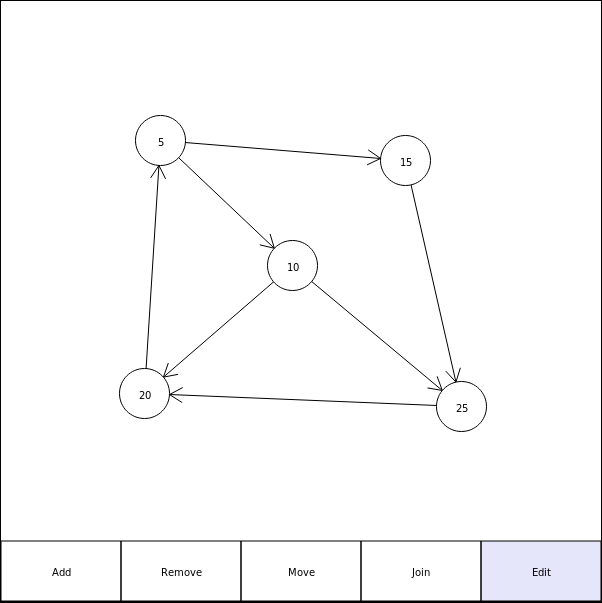
\includegraphics[width=0.75\linewidth]{/graphdrawer/graph0ui}
    \caption{Graph0 - user interface}
    \label{fig:graphdrawerGraph0UserInterface}
\end{figure}
The Graph0 constructor takes two arguments. The first should be a reference to the GraphDrawer object. The second is an optional configuration object. The following properties can be set from values found in the object.
\begin{enumerate}
    \item \code{exportType}, determines if the drawn graph should be exported as a tree or as a graph. Possible values are \code{"Graph"} and \code{"Tree"}. If no value is given, \code{exportType} is set to \code{"Graph"}.
    \item \code{steps}, contains information about a graph or tree which Graph0 should load. This is typically the solution of a task, which should be displayed step by step.
    \item \code{importType}, determines what kind of object \code{steps} contains. It can either be \code{"Graph"} or \code{"Tree"}.
    \item \code{importSource}, if the \code{importType} is \code{"Tree"} then the \code{importSource} property needs to have information about where the tree originated from. If it came from one of the algoritms, it should have the value \code{"Algorithm"}. If a user drew the tree, then it needs to be \code{"Student"} instead.
    \item \code{subType}, determines what kind of algorithm to use. Possible values are \code{"Dijkstra"}. If no value is given, \code{subType} is set to \code{undefined} and no algorithm will be used.
    \item \code{startNodeColor}, determines which fill color the start node is marked with. If no value is given, \code{startNodeColor} is set to a light green color.
    \item \code{endNodeColor}, determines which fill color the end node is marked with. If no value is given, \code{endNodeColor} is set to a light red color.
\end{enumerate}
The Graph0 controller defines five different states, Add, Remove, Move, Join and Edit. Each of them have their own event handler defined by a method in the class. There is also a Mark state which is only available to the user if the \code{subType} is set to \code{"Dijkstra"}.
\begin{enumerate}
    \item Add. The Add state lets the user add a new node to the graph. The new node is placed at the position of interaction event. The value of the node is set to a letter if \code{subType} is set to \code{"Dijkstra"}, or 0 if \code{subType} is undefined. The Add state always consumes the event. 
    \item Remove. The Remove state lets the user remove a node or an edge from the graph. If the interaction event happened inside of a node or close to an edge, it is removed and the event is consumed. If nothing was removed, the event is not consumed. If a node is removed, then any edge connecting the node to another node, is also removed.
    \item Move. The Move state lets the user move a node. This is done using a drag and drop motion. When the interaction starts, a reference to the node under the interaction event is stored. When new events are recieved the position of the node is updated to match the position of the event. The event is consumed only if the first event happened inside a node.
    \item Join. The Join state lets the user create an edge between two nodes. This is done using a drag and drop motion. When the interaction starts, a reference to the node under the interaction event is stored. When the interaction ends, the event handler checks if the is a different node under the event. If another node is found, an edge between this node and the first node is created. The event is consumed only if the first event happened inside a node.
    \item Edit. The Edit state lets the user edit the value of a node or of an edge. The event handler starts by checking if there is a node under the interaction event. If a node is found, the user can edit the value. If no node is found, the handler checks if the event is close to an edge. If it is, the value of the edge can be edited. The event is consumed if the user was given the option to edit a value.
    \item Mark. The Mark state lets the user mark nodes as either a start or end node. If a node is found under the interaction event. It's marked value is updated bases on its current value. A unmarked node is marked as the start node. A start node is marked as the end node. A end node is set to unmarked. The event is consumed if a node changed its marked value.
\end{enumerate}
Before any of the import functions can be used, the data which should be imported needs to be placed in the controller property \code{steps}.
Graph0 can import a list of graphs with the \code{\_parseGraphSteps} function. \code{steps} should contain an array of graph objects. If the graph object has the correct format, it will be read and placed into the world. The graph object should have the following properties.
\begin{enumerate}
    \item \code{type}, with its value set to \code{"Complete"}.
    \item \code{nodes}, which should be an array of node objects. The node objects in the array are copied to the world.
    \item \code{edges}, which should be an array of edge objects. The edge objects in the array are copied to the world.
\end{enumerate}
A tree structure can also be imported with the \code{\_parseTreeSteps} function. Importing a tree is more complicated, because the nodes and edges are not available for copying, so they need to be constructed from the tree information instead. To read a tree object, it needs to have the \code{treeInfo}. \code{treeInfo} should contain an array of tree roots. If there are more than one root, only one of them is added to the world. Buttons which let the user navigate between different trees are added.